\documentclass[a4paper,12pt]{article}

\usepackage[utf8]{inputenc}
\usepackage[english]{babel}
\usepackage{hyperref}
\usepackage{fontenc}
\usepackage{graphicx}
\usepackage{makeidx}
\usepackage{color}
\usepackage{multirow}
\usepackage{tabularx}
\usepackage{longtable}
\usepackage{url}
\usepackage{titlesec}
\usepackage{listings}
\usepackage{xcolor}
\usepackage{colortbl}
\usepackage{geometry}

\geometry{
    a4paper,
    left=25mm,
    right=25mm,
    top=30mm,
    bottom=30mm,
 }

%%%%%%%%%%%%%%%%%%%%%%%%%%%%%
%%%%%%% CONFIGURATION %%%%%%%
%%%%%%%%%%%%%%%%%%%%%%%%%%%%%
%%%%%%%%%%%%%%%%%%%%%%%%%%%%%%%%%%%%%%
%%%%%%% SECTION CONFIGURATIONS %%%%%%%
%%%%%%%%%%%%%%%%%%%%%%%%%%%%%%%%%%%%%%
\newcommand{\sectionbreak}{\clearpage}

\setcounter{secnumdepth}{5}

\titleformat{\paragraph}
{\normalfont\normalsize\bfseries}{\theparagraph}{1em}{}
\titlespacing*{\paragraph}
{0pt}{3.25ex plus 1ex minus .2ex}{1.5ex plus .2ex}


%%%%%%%%%%%%%%%%%%%%%%%%%%%%%%%%%%%%%%
%%%%%%% LISTINGS CONFIGURATION %%%%%%%
%%%%%%%%%%%%%%%%%%%%%%%%%%%%%%%%%%%%%%
\definecolor{mybg}{rgb}{1,1,0.8}
\definecolor{mysoftblue}{rgb}{0.6,0.729,0.867}
\definecolor{mygreen}{rgb}{0,0.6,0}
\definecolor{mygray}{rgb}{0.5,0.5,0.5}
\definecolor{mymauve}{rgb}{0.58,0,0.82}

\lstset{ %
  backgroundcolor=\color{mysoftblue},    % choose the background color; you must add \usepackage{color} or \usepackage{xcolor}
  basicstyle=\ttfamily\scriptsize,        % the size of the fonts that are used for the code
  breakatwhitespace=false,         % sets if automatic breaks should only happen at whitespace
  breaklines=true,                 % sets automatic line breaking
  captionpos=b,                    % sets the caption-position to bottom
  commentstyle=\color{mygreen},    % comment style
  deletekeywords={...},            % if you want to delete keywords from the given language
  escapeinside={\%*}{*)},          % if you want to add LaTeX within your code (example: \%* int v; *) )
  extendedchars=true,              % lets you use non-ASCII characters; for 8-bits encodings only, does not work with UTF-8
  frame=single,                    % adds a frame around the code (none, single)
  keepspaces=true,                 % keeps spaces in text, useful for keeping indentation of code (possibly needs columns=flexible)
  keywordstyle=\color{blue},       % keyword style
  language=Java,                   % the language of the code
  otherkeywords={*,...},           % if you want to add more keywords to the set
  numbers=none,                    % where to put the line-numbers; possible values are (none, left, right)
  numbersep=5pt,                   % how far the line-numbers are from the code
  numberstyle=\tiny\color{mygray}, % the style that is used for the line-numbers
  rulecolor=\color{black},         % if not set, the frame-color may be changed on line-breaks within not-black text (e.g. comments (green here))
  showspaces=false,                % show spaces everywhere adding particular underscores; it overrides 'showstringspaces'
  showstringspaces=false,          % underline spaces within strings only
  showtabs=false,                  % show tabs within strings adding particular underscores
  stepnumber=2,                    % the step between two line-numbers. If it's 1, each line will be numbered
  stringstyle=\color{mymauve},     % string literal style
  tabsize=2,                       % sets default tabsize to 2 spaces
  title=\lstname,                  % show the filename of files included with \lstinputlisting; also try caption instead of title
  aboveskip=20pt,                  % space left avobe the listing
  belowskip=0pt,                   % space left below the listing
  columns=fullflexible             % to allow automatic copy from listings
}


%%%%%%%%%%%%%%%%%%%%%%%%%%%%%%%%%%%
%%%%%%% OTHER CONFIGURATION %%%%%%%
%%%%%%%%%%%%%%%%%%%%%%%%%%%%%%%%%%%

% Horizontal line
\newcommand{\HRule}{
  \rule{\linewidth}{0.5mm}
}

% Color box for comments
\newcommand{\colorComment}[1]{
\begin{table}[h]
    \centering
    \begin{tabular}{p{0.8\textwidth}}
        \cellcolor{orange}\begin{center}
	  #1 \\
        \end{center}
        \\
    \end{tabular}
\end{table}
}
\title{COMP Superscalar}
\author{User Guide: Application execution guide}
\def \compssversion {2.3.rc1807}

\makeindex


%%%%%%%%%%%%%%%%%%%%%%%%%%%%%
%%%%%%%% DOCUMENT %%%%%%%%%%%
%%%%%%%%%%%%%%%%%%%%%%%%%%%%%
\begin{document}

  %%%%%%%%%%%% TITLE PAGE %%%%%%%%%%%%%
  \hypersetup{pageanchor=false}
  \begin{titlepage} 
    \begin{center} 
      
\includegraphics[width=0.3\textwidth]{./Figures/Logos/degradado-naranja-compss.jpg}~\\[1cm] 
      \textsc{\LARGE COMP Superscalar}\\[1.5cm] 
      
      \HRule \\[0.4cm] 
      { \huge \bfseries User Manual \\[0.4cm] }
      { \large \bfseries Application execution guide \\[0.4cm] } 
      \HRule \\[1.5cm] 

      { \large \textsc{Version: \compssversion}} \\[0.3cm]
      { \large \today } 
      
      \vfill 
      % Bottom of the page
      
\includegraphics[width=0.5\textwidth]{./Figures/bsc_280.jpg}~\\[1cm]
    \end{center} 
  \end{titlepage}
  \hypersetup{pageanchor=true}
  
  %%%%%%%% REFERENCE NOTES %%%%%%%%%%
  {
    This manual provides information about how to execute COMPSs applications, how to retrieve the results and the logs of an execution 
    and it provides an overview of the COMPSs tools usage. It is highly recommended to test the examples described in this manual with 
    a working COMPSs installation. For this purpose we provide a \textit{COMPSs Virtual Machine} available at \url{http://compss.bsc.es/} .
    \newline
    
    For information about the installation process please refer to the \textit{COMPSs Installation Guide} available at
    \url{http://compss.bsc.es/} .
    \newline
    
    For further information about the application development please refer to the \textit{COMPSs User Manual: Application development
    guide} available at \url{http://compss.bsc.es/} .
    \newline
    
    For an extensive list of COMPSs application examples (codes, execution commands, results, logs, etc.) please refer to 
    the \textit{COMPSs Sample Applications} guide at \url{http://compss.bsc.es/} .
  }
  
  %%%%%%%% TABLE OF CONTENTS %%%%%%%%%%
  \pagenumbering{roman}
  \setcounter{tocdepth}{6}
  \tableofcontents
  \listoffigures
  %\listoftables
    
  \newpage

  %%%%%%%%%%%%% CONTENTS %%%%%%%%%%%%%%
  \pagenumbering{arabic}
    
  \section{COMP Superscalar (COMPSs)}
\label{sec:Introduction}

COMP Superscalar (COMPSs) is a programming model which aims to ease the development of applications for distributed infrastructures, such as Clusters, Grids and Clouds. COMP superscalar also features a runtime system that exploits the inherent parallelism of applications at execution time.

For the sake of programming productivity, the COMPSs model has four key characteristics:

\begin{itemize}
 
 \item  {\bf Sequential programming:} COMPSs programmers do not need to deal with the typical duties of parallelization and distribution, such as thread creation and synchronization, data distribution, messaging or fault tolerance. Instead, the model is based on sequential programming, which makes it appealing to users that either lack parallel programming expertise or are looking for better programmability.
 
 \item  {\bf Infrastructure unaware:} COMPSs offers a model that abstracts the application from the underlying distributed infrastructure. Hence, COMPSs programs do not include any detail that could tie them to a particular platform, like deployment or resource management. This makes applications portable between infrastructures with diverse characteristics.
 
 \item  {\bf Standard programming languages:} COMPSs is based on the popular programming language Java, but also offers language bindings for Python and C/C++ applications. This facilitates the learning of the model, since programmers can reuse most of their previous knowledge.
 
 \item  {\bf No APIs:} In the case of COMPSs applications in Java, the model does not require to use any special API call, pragma or construct in the application; everything is pure standard Java syntax and libraries. With regard the Python and C/C++ bindings, a small set of API calls should be used on the COMPSs applications.

\end{itemize}


           
  \section{Trace Execution}
\label{sec:Execution}

COMPSs Runtime can generate a post-execution trace of the distributed execution of the application. This trace is useful for
performance analysis and diagnosis.

A trace file may contain different events to determine the COMPSs master state, the task execution state or the file-transfers.
Despite the fact that in the current release we do not support file-transfers, we intend to support them in a near future release.

During the execution of the application, an XML file is created at worker nodes to keep track of 
these events. At the end of the execution, all the XML files are merged to get a final trace file.

In the following sections we explain the command used for tracing, how the events are registered, 
in a process called instrumentation, how to visualize the trace file and make a good analysis of 
performance based on the data shown in the trace.

\subsection{Trace Command}
In order to obtain a post-execution trace file the option \textbf{-t}  must be added to the runcompss command. Next we provide an
example of the command execution with the tracing option enabled for the Hmmer java application.
\begin{lstlisting}[language=bash]
compss@bsc:~$ runcompss -t --classpath=/home/compss/workspace_java/hmmerobj/jar/hmmerobj.jar 
                        hmmerobj.HMMPfam 
                        /sharedDisk/Hmmer/smart.HMMs.bin /sharedDisk/Hmmer/256seq 
                        /home/compss/out.txt 2 8 -A 222
\end{lstlisting}
 

\subsection{Application Instrumentation}
The instrumentation is the process that intercepts different events of the application execution 
and keeps log of them. This will cause an overhead in the execution time of the application that 
the user should take into account, but the collected data will be extremely useful for performance 
analysis and diagnosis.

COMPSs Runtime uses the \textit{Extrae} tool to dynamically instrument the application and the \textit{Paraver} tool to visualize
the obtained tracefiles. Both tools are developped at \textit{BSC} and are available in its webpage \url{http://bsc.es} . 

At the worker nodes, in background, \textit{Extrae} keeps track of the events in an intermediate format 
file (with \textit{.mpit} extension). Inside the master node, at the end of the execution, \textit{Extrae} merges the 
intermediate files to get the final trace file, a \textit{Paraver} format file (.prv). See the visualization 
section \ref{sec:Visualization} in this manual for further information about the \textit{Paraver} tool.

When instrumenting the application \textit{Extrae} will output several messages. At the master node, \textit{Extrae} will show up its
initialization at the begining of the execution and the merging process and the paraver generation at the end of the execution. At the
worker nodes \textit{Extrae} will inform about the intermediate files generation every time a task is executed. Next we provide a 
summary of the \textit{stdout} generated by Hmmer java application execution with the trace flag enabled. 
\begin{lstlisting}[language=bash]
----------------- Executing hmmerobj.HMMPfam --------------------------

WARNING: IT Properties file is null. Setting default values
Welcome to Extrae 3.1.1rc (revision 3360 based on extrae/trunk)
Extrae: Warning! EXTRAE_HOME has not been defined!.
Extrae: Generating intermediate files for Paraver traces.
Extrae: Intermediate files will be stored in /home/compss/workspace_java/hmmerobj/jar
Extrae: Tracing buffer can hold 500000 events
Extrae: Tracing mode is set to: Detail.
Extrae: Successfully initiated with 1 tasks

Extrae: Warning! API tries to initialize more than once
Extrae:          Previous initialization was done by API

[   API]  -  Starting COMPSs Runtime v1.3 (build 20150821-1134.rnull)

...
...
...

[   API]  -  No more tasks for app 1
[   API]  -  Getting Result Files 1
[   API]  -  Execution Finished

Extrae: Intermediate raw trace file created : /home/compss/workspace_java/hmmerobj/jar/set-0/TRACE@bsc.0000031637000000000000.mpit
Extrae: Intermediate raw sym file created : /home/compss/workspace_java/hmmerobj/jar/set-0/TRACE@bsc.0000031637000000000000.sym
Extrae: Deallocating memory.
Extrae: Application has ended. Tracing has been terminated.

merger: Output trace format is: Paraver
merger: Extrae 3.1.1rc (revision 3360 based on extrae/trunk)

mpi2prv: Checking for target directory existance... exists, ok!
mpi2prv: Selected output trace format is Paraver
mpi2prv: Stored trace format is Paraver
mpi2prv: Parsing intermediate files
mpi2prv: Removing temporal files... done
mpi2prv: Congratulations! ./trace/hmmerobj.HMMPfam_compss_trace_1440151114.prv has been generated.

------------------------------------------------------------
\end{lstlisting}

For further information about \textit{Extrae} please visit the following site: 
\begin{center}
\url{http://www.bsc.es/computer-science/extrae} 
\end{center}
          
  \section{Results and logs}
\label{sec:Results_and_Logs}

\subsection{Results}
When executing a user application we consider different type of results:
\begin{itemize}
 \item \textbf{Application Output:} Output generated by the application.
 \item \textbf{Application Files:}  Files used or generated by the application.
 \item \textbf{Tasks Output:} Output generated by the tasks invoked from the application.
\end{itemize}

Regarding the application output, COMPSs will preserve the application output but will add some pre and post output to indicate
the COMPSs Runtime state. Figure \ref{fig:compss_out} shows the standard output generated by the execution of the 
simple java application. The green box highlights the application \textit{stdout} while the rest of the output is produced by COMPSs.  
\begin{figure}[h!]
  \centering
    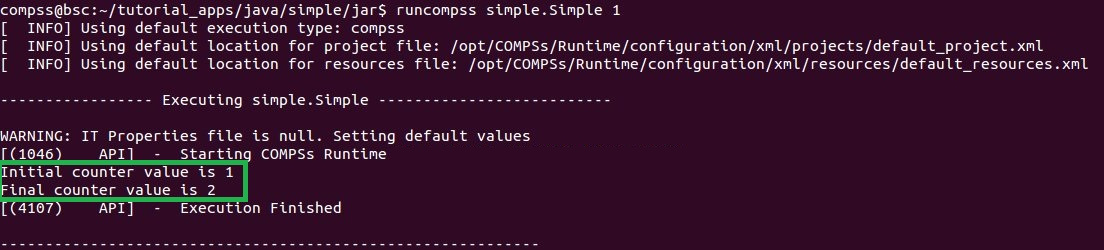
\includegraphics[width=0.95\textwidth]{./Sections/3_Results_and_Logs/Figures/simple_java_stdout.jpeg}
    \caption{Ouput generated by the execution of the \textit{Simple} java application with COMPSs}
    \label{fig:compss_out}
\end{figure}

Regarding the application files, COMPSs \textbf{does not modify} any of them and thus, the
results obtained by executing the application with COMPSs are the same than the ones generated by the sequential execution
of the application.

Regarding the task output, COMPSs does introduce some modifications due to the fact that tasks can be executed in remote
machines. Considering that we call a job the execution of a task in a given resource, after the execution, COMPSs stores 
the \textit{stdout} and the \textit{stderr} of each job inside the \textbf{$/home/\$USER/.COMPSs/\$APPNAME/\$EXEC\_$
$NUMBER/jobs/$}
directory.

Figures \ref{fig:hello_seq} and \ref{fig:hello_compss} show an example of the results obtained from the execution of the \textit{Hello} java 
java application. While Figure \ref{fig:hello_seq} provides the sequential execution of the application, Figure \ref{fig:hello_compss}
provides its equivalent COMPSs execution. Notice that, the sequential execution produces the \" Hello World! (from a task)\" message
in the \textit{stdout} while the COMPSs execution stores the message inside the \textit{$job1\_NEW.out$} file.
\begin{figure}[h!]
  \centering
    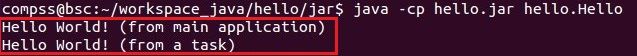
\includegraphics[width=0.7\textwidth]{./Sections/3_Results_and_Logs/Figures/hello_seq_stdout.jpeg}
    \caption{Sequential execution of the \textit{Hello} java application}
    \label{fig:hello_seq}
\end{figure}

\begin{figure}[h!]
  \centering
    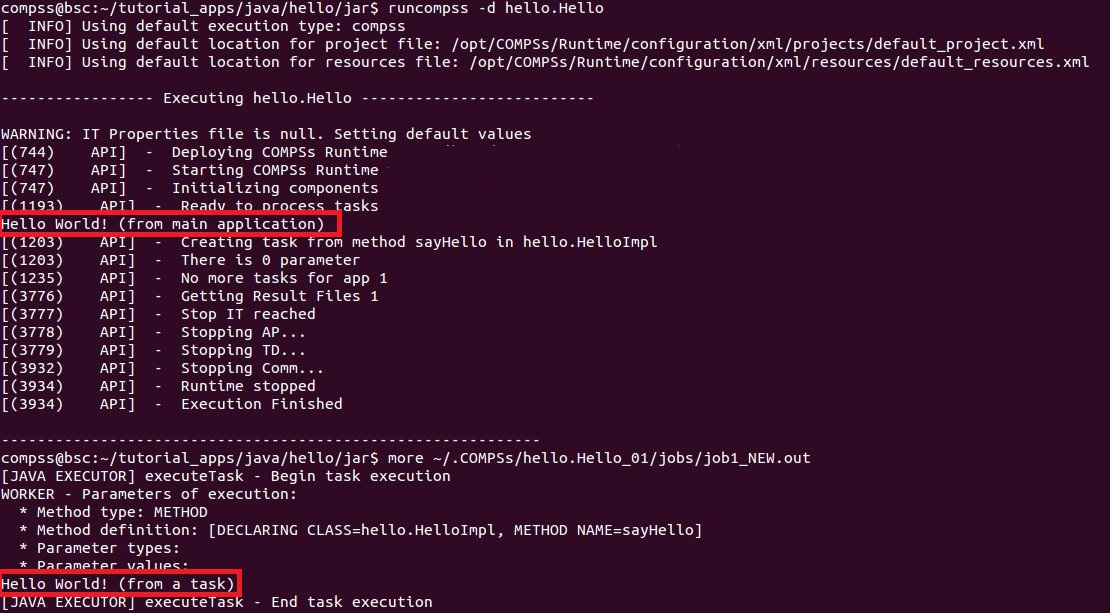
\includegraphics[width=\textwidth]{./Sections/3_Results_and_Logs/Figures/hello_compss_stdout_and_job.jpeg}
    \caption{COMPSs execution of the \textit{Hello} java application}
    \label{fig:hello_compss}
\end{figure}
\newpage

\subsection{Logs}
COMPSs includes three log levels for running applications but users can modify them or add more levels by editing the
logger files under the \textit{/opt/COMPSs/Runtime/configuration/log/} folder. Any of these log levels can be selected by 
adding the \textit{$--log\_level=<debug | info | off >$} flag to the runcompss command. The default value is \textit{off}.

The logs generated by the execution number $NUM\_EXEC$ of the application APP by the user USER are stored under
\textit{$/home/\$USER/.COMPSs/\$APP/\$NUM\_EXEC/$} folder (from this point on: \textbf{base log folder}). The execution number is 
automatically tracked to prevent the loss of data from previous executions, but users do not need to take care of this value. 

When running COMPSs with \textbf{log level off} only the errors are reported. This means that the \textit{base log folder} will 
contain two empty files (\textbf{runtime.log} and \textbf{resources.log}) and one empty folder (\textit{jobs}). If somehow the 
application has failed, the \textit{runtime.log} and/or the \textit{resources.log} will not be empty and a new file per 
failed job will appear inside the \textit{jobs} folder to store the \textit{stdout} and the \textit{stderr}. 
Figure \ref{fig:simple_log_off} shows the logs generated by the execution of the Simple java application (without errors) 
in \textbf{off} mode. 
\begin{figure}[h!]
  \centering
    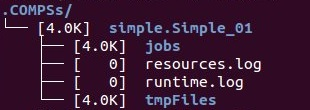
\includegraphics[width=0.4\textwidth]{./Sections/3_Results_and_Logs/Figures/simple_log_off.jpeg}
    \caption{Structure of the logs folder for the Simple java application in \textbf{off} mode}
    \label{fig:simple_log_off}
\end{figure}

When running COMPSs with \textbf{log level info} the \textit{base log folder} will contain two files (\textbf{runtime.log} and 
\textbf{resources.log}) and one folder (\textit{jobs}). The \textbf{runtime.log} file contains the execution information retrieved 
from the master resource; including the file transfers and the job submission details. The \textbf{resources.log} file contains 
information about the available resources such as the number of processors of each resource (slots), the information about running or 
pending tasks in the resource queue and the created and destroyed resources. The jobs folder will be empty unless there has been a
failed job. In this case, for each failed job, it will store one file for the \textit{stdout} and another for the \textit{stderr}.
As an example, Figure \ref{fig:simple_log_info} shows the logs generated by the same execution than the previous case 
but with \textbf{info} mode. 
\begin{figure}[h!]
  \centering
    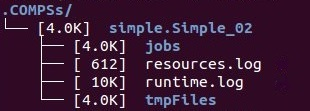
\includegraphics[width=0.4\textwidth]{./Sections/3_Results_and_Logs/Figures/simple_log_info.jpeg}
    \caption{Structure of the logs folder for the Simple java application in \textbf{info} mode}
    \label{fig:simple_log_info}
\end{figure}

The runtime.log and resources.log are quite large files and, thus, should be only checked by advanced users. For an
easier interpretation of these files the COMPSs Framework includes a monitor tool. For further information about the COMPSs Monitor
please check Section \ref{subsec:monitor}.

Figures \ref{fig:simple_runtimelog} and \ref{fig:simple_resourceslog} provide the content of these two files generated
by the execution of the \textit{Simple} java application. 
\begin{figure}[h!]
  \centering
    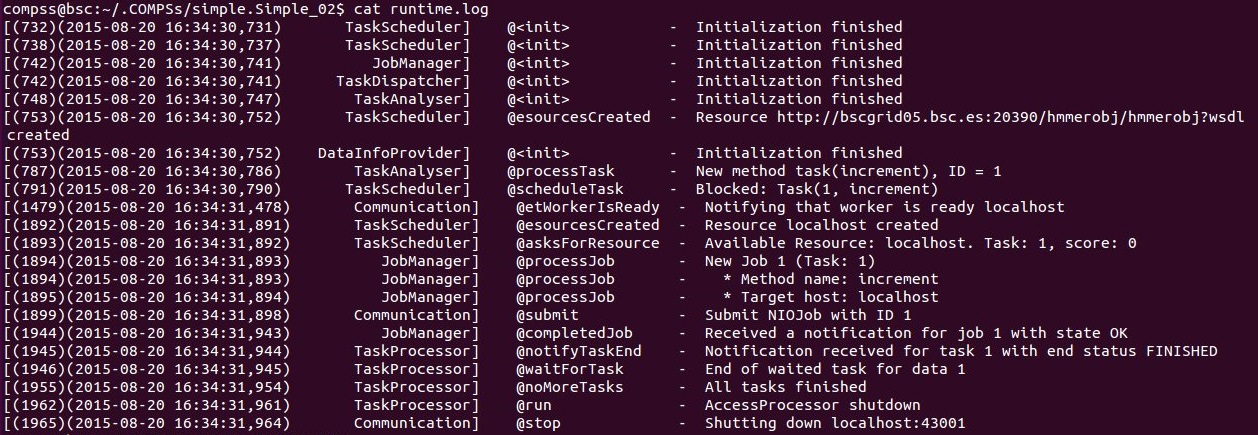
\includegraphics[width=0.95\textwidth]{./Sections/3_Results_and_Logs/Figures/simple_runtimelog.jpeg}
    \caption{runtime.log generated by the execution of the \textit{Simple} java application}
    \label{fig:simple_runtimelog}
\end{figure}

\begin{figure}[h!]
  \centering
    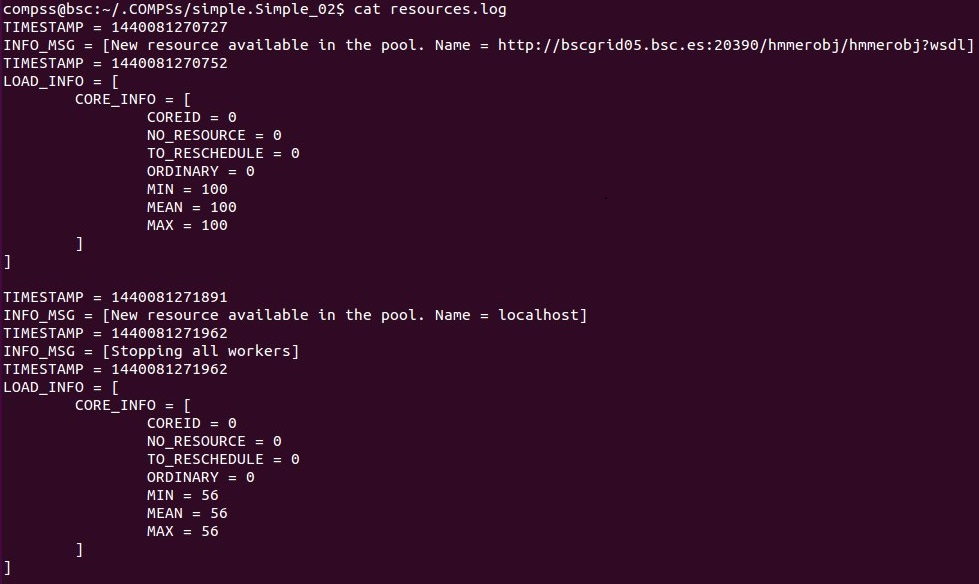
\includegraphics[width=0.95\textwidth]{./Sections/3_Results_and_Logs/Figures/simple_resourceslog.jpeg}
    \caption{resources.log generated by the execution of the \textit{Simple} java application}
    \label{fig:simple_resourceslog}
\end{figure}

Running COMPSs with \textbf{log level debug} generates the same files as the info log level but with more detailed information.
Additionally, the \textit{jobs} folder contains two files per \textbf{submitted} job; one for the \textit{stdout} and another for
the \textit{stderr}. In the other hand, the COMPSs Runtime state is printed out on the \textit{stdout}. Figure 
\ref{fig:simple_log_debug} shows the logs generated by the same execution than the previous cases 
but with \textbf{debug} mode. 

The runtime.log and the resources.log files generated in this mode can be \textbf{extremely large}. Consequently, the users should
take care of their quota and manually and erase these files if needed. \newline

\begin{figure}[h!]
  \centering
    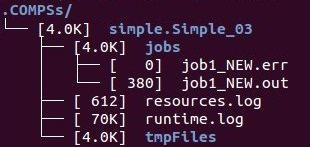
\includegraphics[width=0.4\textwidth]{./Sections/3_Results_and_Logs/Figures/simple_log_debug.jpeg}
    \caption{Structure of the logs folder for the Simple java application in \textbf{debug} mode}
    \label{fig:simple_log_debug}
\end{figure}

Furthermore, when running other runcompss flags (such as monitoring or tracing) additional folders will appear inside the 
\textit{base log folder}. The meaning of the files inside these folders is explained in Section \ref{sec:Tools}. 

           
  \section{COMPSs Tools}
\label{sec:Tools}

%%%%%%%%%%%%%%%%%%%%%%%%%%%%%%%%%%%%%%%%%%%%%%%%%%%%%%%
%%%%%%%%%%%%%%%%% APPLICATION GRAPH %%%%%%%%%%%%%%%%%%%
%%%%%%%%%%%%%%%%%%%%%%%%%%%%%%%%%%%%%%%%%%%%%%%%%%%%%%%
\subsection{Application graph}
At the end of the application execution a dependency graph can be generated representing the order of execution of each type of 
task and their dependencies. To allow the final graph generation the \textit{-g} flag has to be passed to the \textit{runcompss} command; the graph file is written in the \textit{$base\_log\_folder$}$/monitor/complete\_graph$.dot at the end of the execution.

Figure \ref{fig:complete_graph} shows a dependency graph example of a \textit{SparseLU} java application. The graph can be
visualized by running the following command:
\begin{lstlisting}[language=bash]
compss@bsc:~$ gengraph ~/.COMPSs/sparseLU.arrays.SparseLU_01/monitor/complete_graph.dot
\end{lstlisting}

\begin{figure}[h!]
  \centering
    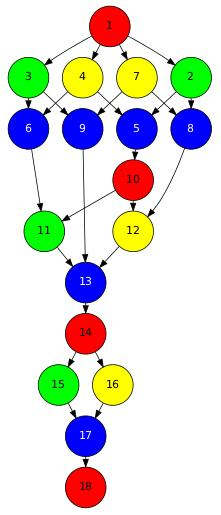
\includegraphics[width=0.3\textwidth]{./Sections/4_Tools/Figures/dependency_graph.jpeg}
    \caption{The dependency graph of the SparseLU application}
    \label{fig:complete_graph}
\end{figure}



%%%%%%%%%%%%%%%%%%%%%%%%%%%%%%%%%%%%%%%%%%%%%%%%%%%%%%%
%%%%%%%%%%%%%%%%%%%%%%%% MONITOR %%%%%%%%%%%%%%%%%%%%%%
%%%%%%%%%%%%%%%%%%%%%%%%%%%%%%%%%%%%%%%%%%%%%%%%%%%%%%%
\subsection{COMPSs Monitor}
\label{subsec:monitor}
The COMPSs Framework includes a Web graphical interface that can be used to monitor the execution of COMPSs applications. COMPSs Monitor is installed as a service and can be easily managed by running any of the following
commands:
\begin{lstlisting}[language=bash]
compss@bsc:~$ /etc/init.d/compss-monitor usage
Usage: compss-monitor {start | stop | reload | restart | try-restart | force-reload | status}
\end{lstlisting}

\subsubsection{Service configuration}
The COMPSs Monitor service can be configured by editing the \textit{/opt/COMPSs/Tools/}
\textit{monitor/apache-tomcat/conf/compss-monitor.conf}
file which contains one line per property:
\begin{itemize}
 \item \textbf{$IT\_MONITOR$} Default directory to retrieve monitored applications (defaults to the \textit{.COMPSs} folder inside the \textit{root} user).
 \item \textbf{$COMPSs\_MONITOR\_PORT$} Port where to run the compss-monitor web service (defaults to 8080).
 \item \textbf{$COMPSs\_MONITOR\_TIMEOUT$} Web page timeout between browser and server (defaults to 20s).
\end{itemize}

\subsubsection{Usage}
In order to use the COMPSs Monitor users need to start the service as shown in Figure \ref{fig:monitor_start}.
\begin{figure}[thb!]
  \centering
    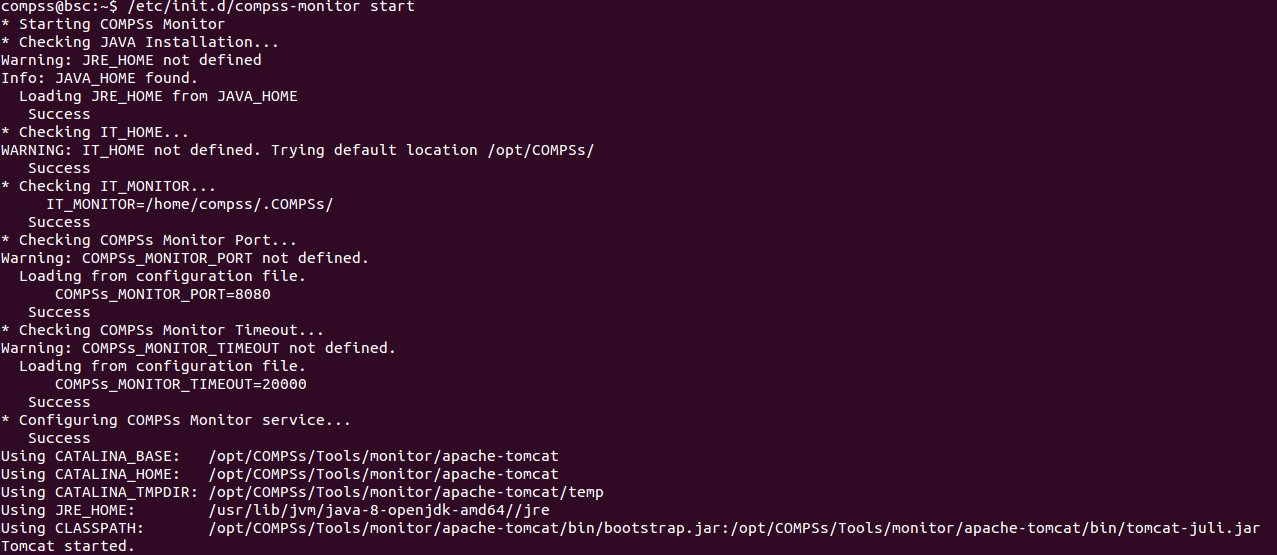
\includegraphics[width=\textwidth]{./Sections/4_Tools/Figures/monitor_start.jpeg}
    \caption{COMPSs Monitor start command}
    \label{fig:monitor_start}
\end{figure}

And use a web browser to open the specific URL:
\begin{lstlisting}[language=bash]
compss@bsc:~$ firefox http://localhost:8080/compss-monitor &
\end{lstlisting}

The COMPSs Monitor allows to monitor applications from different users and thus, users need to first login to access their applications. As shown in Figure \ref{fig:monitoring_interface}, the users can select any of their executed or running COMPSs applications and display it.
\begin{figure}[thb!]
  \centering
    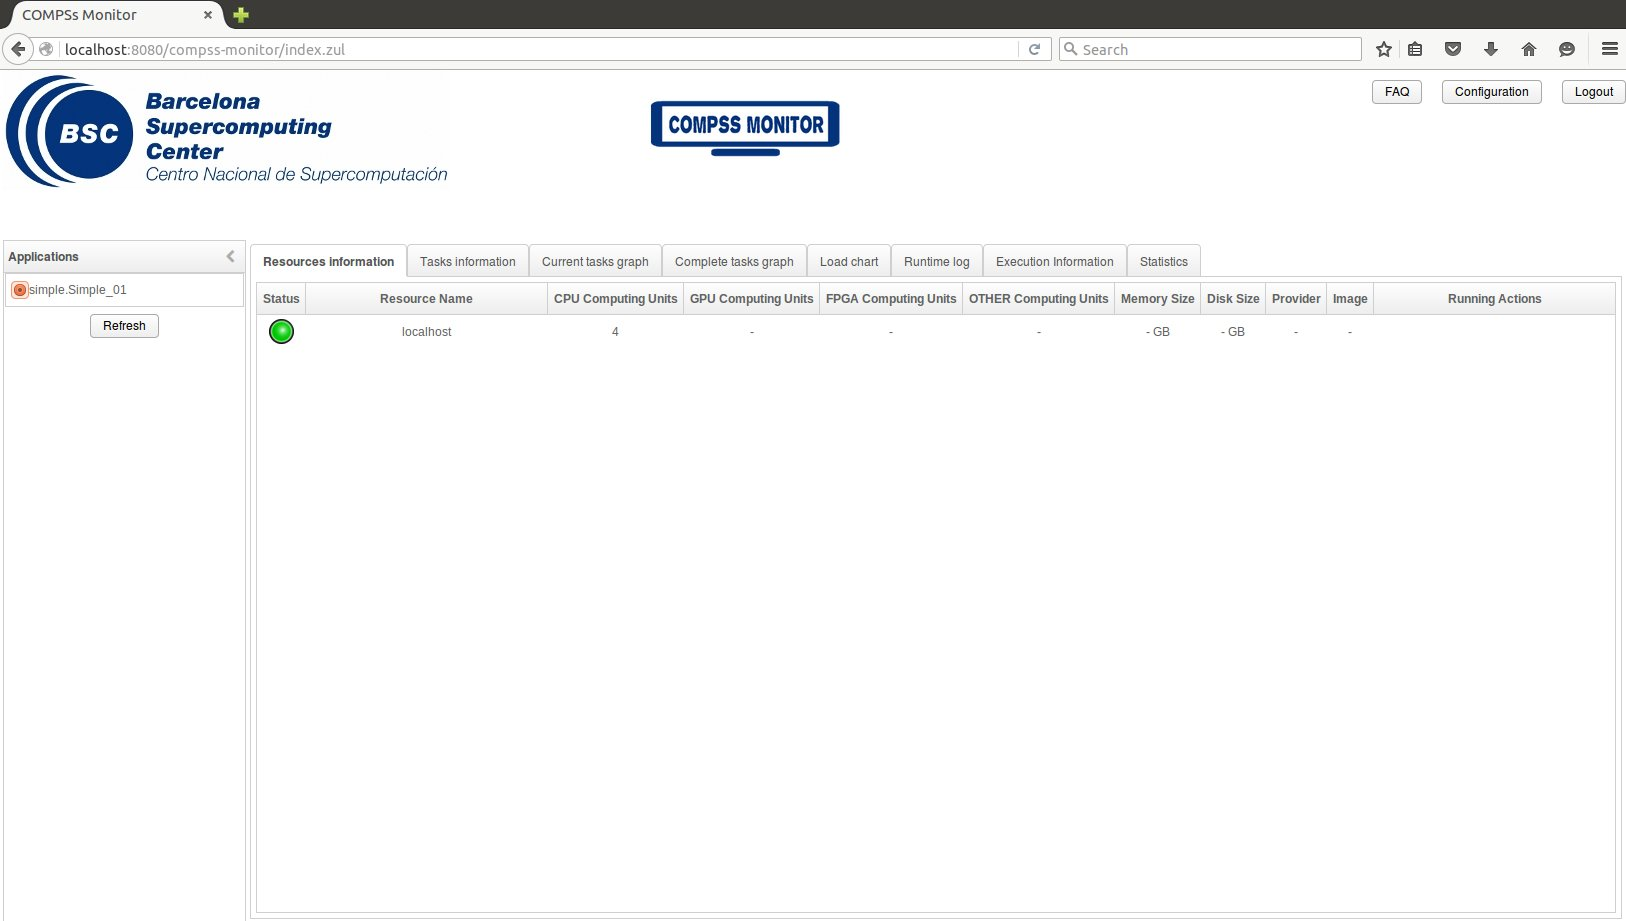
\includegraphics[width=0.95\textwidth]{./Sections/4_Tools/Figures/compss_monitor.jpeg}
    \caption{COMPSs monitoring interface}
    \label{fig:monitoring_interface}
\end{figure}

To enable \textbf{all} the COMPSs Monitor features, applications must run the runcompss command with the \textit{-m} flag. This flag 
allows the  COMPSs Runtime to store special information inside inside the \textit{log base folder} under the \textit{monitor} 
folder (see Figures \ref{fig:simple_exec_monitor} and \ref{fig:simple_logs_monitor}). Only advanced users should modify or delete any of these files. If the application that a user is trying to monitor 
has not been executed with this flag, some of the COMPSs Monitor features will be disabled. 
\begin{figure}[ht!]
  \centering
    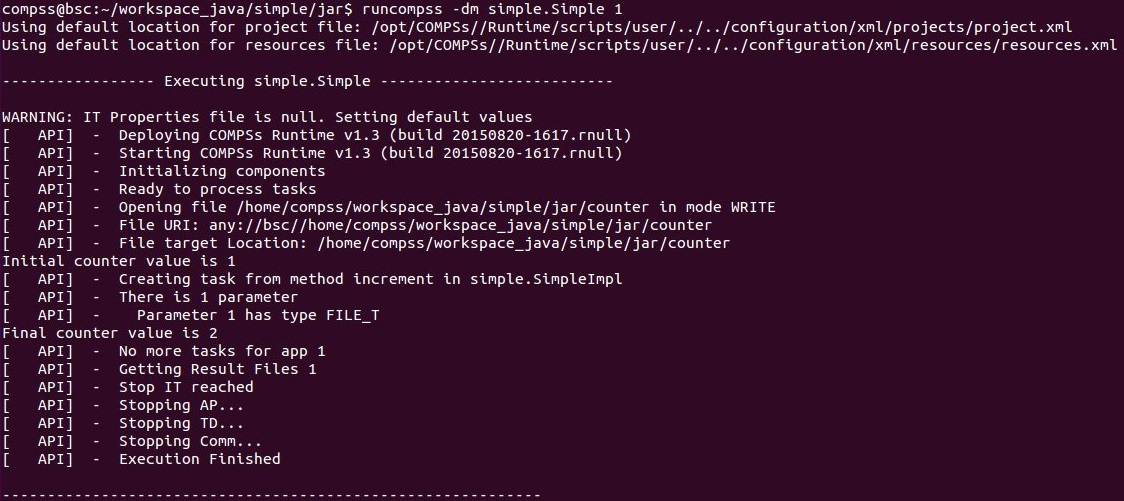
\includegraphics[width=0.95\textwidth]{./Sections/4_Tools/Figures/simple_monitor.jpeg}
    \caption{Execution of the Simple Java application with the monitoring flag enabled}
    \label{fig:simple_exec_monitor}
\end{figure}

\begin{figure}[ht!]
  \centering
    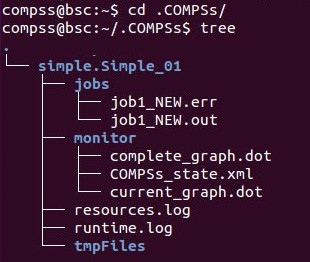
\includegraphics[width=0.4\textwidth]{./Sections/4_Tools/Figures/logs_with_monitor.jpeg}
    \caption{Logs generated by the Simple java application with the monitoring flag enabled}
    \label{fig:simple_logs_monitor}
\end{figure}

\newpage
\subsubsection{Graphical Interface features}
In this section we provide a summary of the COMPSs Monitor supported features available through the graphical interface:
\begin{itemize}
 \item \textbf{Resources information} \newline
	Provides information about the resources used by the application
 \item \textbf{Tasks information} \newline
	Provides information about the tasks definition used by the application
 \item \textbf{Current tasks graph} \newline
	Shows the tasks dependency graph currently stored into the COMPSs Runtime
 \item \textbf{Complete tasks graph} \newline
	Shows the complete tasks dependecy graph of the application
 \item \textbf{Load chart} \newline
	Shows different dynamic charts representing the evolution over time of the resources load and the tasks load
 \item \textbf{Runtime log} \newline
	Shows the runtime log
 \item \textbf{Execution Information} \newline
	Shows specific job information allowing users to easily select failed or uncompleted jobs
 \item \textbf{Statistics} \newline
	Shows application statistics such as the accumulated cloud cost. 
\end{itemize}

\colorComment{\textbf{Attention}: To enable all the COMPSs Monitor features applications must run with the \textit{$-m$} flag.}

The webpage also allows users to configure some performance parameters of the monitoring service by accessing the 
\textit{Configuration} button at the top-right corner of the web page. 

For specific COMPSs Monitor feature configuration please check our \textit{FAQ} section at the top-right corner of the web page. 


%%%%%%%%%%%%%%%%%%%%%%%%%%%%%%%%%%%%%%%%%%%%%%%%%%%%%%%
%%%%%%%%%%%%%%%% APPLICATION TRACING %%%%%%%%%%%%%%%%%%
%%%%%%%%%%%%%%%%%%%%%%%%%%%%%%%%%%%%%%%%%%%%%%%%%%%%%%%
\subsection{Application tracing}
\label{sec:Tracing}
COMPSs Runtime can generate a post-execution trace of the execution of the application. This trace is useful for
performance analysis and diagnosis.

A trace file may contain different events to determine the COMPSs master state, the task execution state or the file-transfers.
The current release does not support file-transfers informations.

During the execution of the application, an XML file is created in the worker nodes to keep track of 
these events. At the end of the execution, all the XML files are merged to get a final trace file.

In this manual we only provide information about how to obtain a trace and about the available Paraver (the tool used to analyze the traces) configurations. For further
information about the application instrumentation or the trace visualization and configurations please check the \textit{COMPSs Tracing Manual} 
available at \url{http://compss.bsc.es} .

\subsubsection{Trace Command}


In order to obtain a post-execution trace file one of the following options \textbf{-t, -{}-tracing, -{}-tracing=true, -{}-tracing=basic} 
must be added to the runcompss command. All this options activate the basic tracing mode; the advanced mode is activated with the 
option \textbf{-{}-tracing=advanced}. For further information about advanced mode check the \textit{COMPSs Tracing Manual}. Next, we
provide an example of the command execution with the basic tracing option enabled for a java K-Means application.

\begin{lstlisting}[language=bash]
compss@bsc:~$ runcompss -t kmeans.Kmeans
*** RUNNING JAVA APPLICATION KMEANS
Resolved: /path/to/jar/kmeans.jar:

----------------- Executing kmeans.Kmeans --------------------------

Welcome to Extrae 3.3.0 (revision 3966 based on extrae/trunk)
Extrae: Parsing the configuration file (/opt/COMPSs/Runtime/configuration/xml/tracing/extrae_basic.xml) begins
Extrae: Tracing package is located on /opt/COMPSs/Dependencies/extrae/
Extrae: Generating intermediate files for Paraver traces.
Extrae: PAPI domain set to USER for HWC set 1
Extrae: HWC set 1 contains following counters < PAPI_TOT_INS (0x80000032) PAPI_TOT_CYC (0x8000003b) PAPI_LD_INS (0x80000035) PAPI_SR_INS (0x80000036) > - changing every 500000000 nanoseconds
Extrae: PAPI domain set to USER for HWC set 2
Extrae: HWC set 2 contains following counters < PAPI_TOT_INS (0x80000032) PAPI_TOT_CYC (0x8000003b) PAPI_LD_INS (0x80000035) PAPI_SR_INS (0x80000036) PAPI_L2_DCM (0x80000002) > - changing every 500000000 nanoseconds
WARNING: IT Properties file is null. Setting default values
[(751)    API]  -  Deploying COMPSs Runtime v2.0 (build 20161114-1231)
[(753)    API]  -  Starting COMPSs Runtime v2.0 (build 20161114-1231)
[(753)    API]  -  Initializing components
[(1142)   API]  -  Ready to process tasks
...
...
...
merger: Output trace format is: Paraver
merger: Extrae 3.3.0 (revision 3966 based on extrae/trunk)
mpi2prv: Assigned nodes < Marginis >
mpi2prv: Assigned size per processor < <1 Mbyte >
mpi2prv: File set-0/TRACE@Marginis.0000001904000000000000.mpit is object 1.1.1 on node Marginis assigned to processor 0
mpi2prv: File set-0/TRACE@Marginis.0000001904000000000001.mpit is object 1.1.2 on node Marginis assigned to processor 0
mpi2prv: File set-0/TRACE@Marginis.0000001904000000000002.mpit is object 1.1.3 on node Marginis assigned to processor 0
mpi2prv: File set-0/TRACE@Marginis.0000001980000001000000.mpit is object 1.2.1 on node Marginis assigned to processor 0
mpi2prv: File set-0/TRACE@Marginis.0000001980000001000001.mpit is object 1.2.2 on node Marginis assigned to processor 0
mpi2prv: File set-0/TRACE@Marginis.0000001980000001000002.mpit is object 1.2.3 on node Marginis assigned to processor 0
mpi2prv: File set-0/TRACE@Marginis.0000001980000001000003.mpit is object 1.2.4 on node Marginis assigned to processor 0
mpi2prv: File set-0/TRACE@Marginis.0000001980000001000004.mpit is object 1.2.5 on node Marginis assigned to processor 0
mpi2prv: Time synchronization has been turned off
mpi2prv: A total of 9 symbols were imported from TRACE.sym file
mpi2prv: 0 function symbols imported
mpi2prv: 9 HWC counter descriptions imported
mpi2prv: Checking for target directory existance... exists, ok!
mpi2prv: Selected output trace format is Paraver
mpi2prv: Stored trace format is Paraver
mpi2prv: Searching synchronization points... done
mpi2prv: Time Synchronization disabled.
mpi2prv: Circular buffer enabled at tracing time? NO
mpi2prv: Parsing intermediate files
mpi2prv: Progress 1 of 2 ... 5% 10% 15% 20% 25% 30% 35% 40% 45% 50% 55% 60% 65% 70% 75% 80% 85% 90% 95% done
mpi2prv: Processor 0 succeeded to translate its assigned files
mpi2prv: Elapsed time translating files: 0 hours 0 minutes 0 seconds
mpi2prv: Elapsed time sorting addresses: 0 hours 0 minutes 0 seconds
mpi2prv: Generating tracefile (intermediate buffers of 838848 events)
         This process can take a while. Please, be patient.
mpi2prv: Progress 2 of 2 ... 5% 10% 15% 20% 25% 30% 35% 40% 45% 50% 55% 60% 65% 70% 75% 80% 85% 90% 95% done
mpi2prv: Warning! Clock accuracy seems to be in microseconds instead of nanoseconds.
mpi2prv: Elapsed time merge step: 0 hours 0 minutes 0 seconds
mpi2prv: Resulting tracefile occupies 991743 bytes
mpi2prv: Removing temporal files... done
mpi2prv: Elapsed time removing temporal files: 0 hours 0 minutes 0 seconds
mpi2prv: Congratulations! ./trace/kmeans.Kmeans_compss_trace_1460456106.prv has been generated.
[   API]  -  Execution Finished
\end{lstlisting}

At the end of the execution the trace will be stored inside the \textit{trace} folder under the application log directory.
\begin{lstlisting}[language=bash]
compss@bsc:~$ cd .COMPSs/kmeans.Kmeans_01/trace/
compss@bsc:~$ ls -1
kmeans.Kmeans_compss_trace_1460456106.pcf
kmeans.Kmeans_compss_trace_1460456106.prv
kmeans.Kmeans_compss_trace_1460456106.row
\end{lstlisting}


\subsubsection{Trace visualization}
The traces generated by an application execution are ready to be visualized with \textit{Paraver}. \textit{Paraver} is a powerful 
tool developed by \textit{BSC} that allows users to show many views of the trace data by means of different configuration files.
Users can manually load, edit or create configuration files to obtain different trace data views.

If \textit{Paraver} is installed, issue the following command to visualize a given tracefile:

\begin{lstlisting}[language=bash]
compss@bsc:~$ wxparaver path/to/trace/trace_name.prv
\end{lstlisting}

For further information about \textit{Paraver} please visit the following site:
\begin{center}
\url{http://www.bsc.es/computer-sciences/performance-tools/paraver}
\end{center}

\newpage

%%%%%%%%%%%%%%%%%%%%%%%%%%%%%%%%%%%%%%%%%%%%%%%%%%%%%%%
%%%%%%%%%%%%%%%%%%%%%%%%% IDE %%%%%%%%%%%%%%%%%%%%%%%%%
%%%%%%%%%%%%%%%%%%%%%%%%%%%%%%%%%%%%%%%%%%%%%%%%%%%%%%%
\subsection{COMPSs IDE}
\label{subsec:IDE}
COMPSs IDE is an Integrated Development Environment to develop, compile, deploy and execute COMPSs applications. It is available
through the \textit{Eclipse Market} as a plugin and provides an even easier way to work with COMPSs.

For further information please check the \textit{COMPSs IDE User Guide} available at: \url{http://compss.bsc.es} .

  
  \section{Special Execution Platforms}
\label{sec:Execution_Platfors}

This section provides information about how to run COMPSs Applications in specific platforms such as \textit{Docker},
\textit{Chameleon} or \textit{MareNostrum}.


%%%%%%%%%%%%%%%%%%%%%%%%%%%%%%%%%%%%%%%%%
%% DOCKERS
%%%%%%%%%%%%%%%%%%%%%%%%%%%%%%%%%%%%%%%%%
\subsection{Docker}

\subsubsection{Introduction}
Docker is an open-source project that automates the deployment of applications inside software containers, 
by providing an additional layer of abstraction and automation of operating-system-level virtualization on Linux.
In addition to the Docker container engine, there are other Docker tools that allow users to create complex applications (Docker-Compose) 
or to manage a cluster of Docker containers (Docker Swarm).
\\ \\ 
COMPSs supports running a distributed application in a Docker swarm cluster.
\\

\subsubsection{Requirements}
In order to use COMPSs with Docker, some requirements must be fulfilled:
\begin{itemize}  
\item Have \textbf{Docker} and \textbf{Docker-Compose} installed in your local machine.
\item Have an available \textbf{Docker swarm cluster} and its swarm manager ip and port to access it remotely.
\item A \textbf{Dockerhub account}. Dockerhub is an online repository for Docker images. We don't currently support
      another sharing method besides uploading to Dockerhub, so you will need to provide a username.
      This has the advantage that it takes very little to upload the image, since Dockerhub 
      will just need the delta layers from the base image of COMPSs.
\end{itemize}

For more information about Docker and how to install different components, visit Docker site: \url{https://www.docker.com/}

\clearpage
\subsubsection{Execution}
To execute COMPSs in a Docker swarm cluster, you must use the \textbf{runcompss-docker} command, instead of runcompss.
\\
The command \textbf{runcompss-docker} has some \textbf{additional arguments} that will be needed by COMPSs to run your application 
in a distributed Docker swarm cluster environment.
The rest of typical arguments (classpath, project, etc.) will be delegated to runcompss command.
\\ \\
These \textbf{mandatory} additional arguments must go \textbf{before} the typical runcompss arguments. 
The \textbf{runcompss-docker additional arguments} are:
\begin{itemize}
 \item { 
 \textbf{-{}-w, -{}-worker-containers:} \\  
 Specifies the number of \textbf{worker containers} the app will execute on. One more container will be created to host the \textbf{master}. 
 If you have enough nodes in the swarm cluster, each container will be executed by one node.\\
 Example:  \textbf{-{}-worker-containers=3}
 }
 
 \item { 
 \textbf{-{}-c, -{}-context-dir:} \\
 Specifies the \textbf{context directory} of the app. 
 The context directory is a local directory that \textbf{must contain the needed binaries and input files of the app}.
 In its simplest case, it will contain the executable file (a .jar for example).
 Take into account that you should not put unnecessary files in the context-directory, 
 since \textbf{it will be copied to all the nodes} that need it.
 
 Example: \textbf{-{}-context-dir='/home/compss-user/my-app-dir'}, where my-app-dir contains 'app.jar', 'data1.dat' and 'data2.csv', for example.
 }

 \item { 
 \textbf{-{}-s, -{}-swarm-manager:} \\
 Specifies the swarm manager ip and port (format: <ip>:<port>). 
 You can test if the swarm manager really works and is reachable from your machine
 running from your machine the Docker hello-world container.\\
 Example: \textbf{-{}-swarm-manager='129.114.108.8:4000'}
 }
 
 \item { 
 \textbf{-{}-u, -{}-username:} \\
 Specifies a \textbf{Dockerhub username}, to upload the app image, so the workers can pull it in runtime. 
 As stated in the requirements sections, this is needed to share your container application image with the nodes that need it.
 }
\end{itemize}

As an \textbf{optional} argument:
\begin{itemize}
 \item { 
 \textbf{-{}-n, -{}-no-refresh-app-image:} \\
 If this flag is on, the \textbf{app image won't be uploaded }to Dockerhub.
 Workers won't pull the image either.
 Use this flag if the application has not changed since the last running.
 This way the execution will be \textbf{faster}, and you won't need to specify the Dockerhub username nor write its password.
 But remember! If you make any change to the application, run an execution without this flag at least once, 
 to update the online application image.
 }
\end{itemize}

Here is the \textbf{format} you must use with \textbf{runcompss-docker} command:
\begin{lstlisting}[language=bash]
runcompss-docker --worker-containers=N 
                 --context-dir='CTX_DIR'
                 --swarm-manager='<ip>:<port>'
                 --username='dockerhub_username'
                 [rest of classic runcompss args]
\end{lstlisting}           

Or alternatively, in its shortest form:
\begin{lstlisting}[language=bash]
runcompss-docker --w=N  --c='CTX_DIR' --s='<ip>:<port>' --u='dockerhub_username' 
                 [rest of classic runcompss args]
\end{lstlisting}        

The runcompss-docker command creates a Docker image from a common COMPSs docker image by adding your context directory to it. 
Then it uploads this image to Dockerhub and Docker Compose is in charge of spawning the different application containers to the docker swarm manager.
Then the Docker Swarm starts the containers and the application.
\\
The COMPSs Docker base image is available in the Dockerhub. In case you need it, you can pull it using the following command:
\begin{lstlisting}[language=bash]
docker pull compss/compss
\end{lstlisting}

\clearpage
\subsubsection{Execution with TLS}
If your cluster uses \textbf{TLS} or has been created using \textbf{Docker-Machine}, you will have to 
\textbf{export two environment variables} before using runcompss-docker:\\ \\
On one hand, \textbf{DOCKER\_TLS\_VERIFY} environment variable will tell Docker that you are using TLS:
\begin{lstlisting}[language=bash]
export DOCKER_TLS_VERIFY="1"
\end{lstlisting}
On the other hand, \textbf{DOCKER\_CERT\_PATH} variable will tell Docker where to find your TLS certificates. As an example:
\begin{lstlisting}[language=bash]
export DOCKER_CERT_PATH="/home/compss-user/.docker/machine/machines/my-manager-node"
\end{lstlisting}

In case you have created your cluster using docker-machine, in order to know what
your \textit{DOCKER\_CERT\_PATH} is, you can use this command:
\begin{lstlisting}[language=bash]
docker-machine env my-swarm-manager-node-name | grep DOCKER_CERT_PATH
\end{lstlisting}
In which \textit{swarm-manager-node-name} must be changed by the name docker-machine has assigned to your swarm manager node.\\ \\
With these environment variables set, you are ready to use \textbf{runcompss-docker} in a cluster using TLS.

\clearpage
\subsubsection{Execution results}
The execution results will be retrieved from the master container of your application.
\\ \\ 
If your context-directory name is \textbf{'matmul'}, then your results will be saved in the \textbf{'matmul-results'} directory, 
which \textbf{is located in the SAME directory as your context-directory is in}. 
\\ \\ 
Inside the \textbf{'matmul-results'} directory you will have:
\begin{itemize}
 \item  A folder named \textbf{'matmul'} with all the result files that were
	in the same directory as the executable when the application execution ended.  
	More precisely, this will contain the context-directory state right after finishing your application execution.
	\\
	\\
	Additionally, and for more advanced debug purposes,
	you will have some intermidiate files created by runcompss-docker(Dockerfile, project.xml, resources.xml),
	in case you want to check for more complex errors or details. 
	
	
  \item A folder named \textbf{'debug'}, which (in case you used the runcompss debug option (\textbf{-d})), 
        will contain the \textbf{'.COMPSs'} directory, which contains another directory in which there are the typical debug files runtime.log, jobs, etc.
	\\
        Remember \textbf{.COMPSs} is a \textbf{hidden} directory, take this into account if you do \textbf{ls} inside the debug directory (add the \textbf{-a} option).
  
\end{itemize}

To make it simpler, we provide a \textbf{tree visualization} of an example of what your directories should look like after the execution.
In this case we executed the \textbf{Matmul example application} that we provide you:
\\*
\\*
\\*
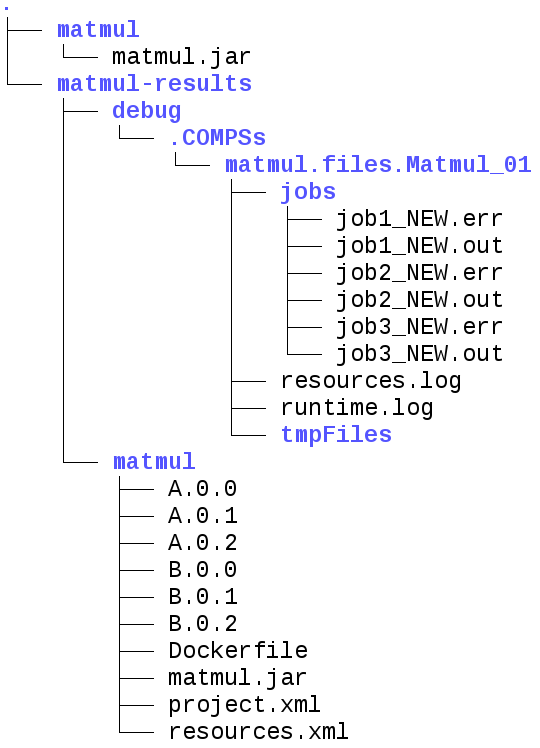
\includegraphics[width=0.3\textwidth]{./Sections/5_Execution_Platforms/Figures/docker-matmul-results-tree.png} 

\clearpage
\subsubsection{Execution examples}
And here is one example to run the Matmul example application. 
In this case, we are specifying:

\begin{itemize}  
\item Use \textbf{5 worker docker containers}. They will be distributed amongst the swarm cluster nodes as balanced as possible.
\item The \textbf{context directory} will be '/home/compss-user/my-app-dir'.
\item The \textbf{swarm-manager ip} will be 129.114.108.8, with the swarm manager located in the \textbf{port} 4000.
\item The \textbf{Dockerhub username} will be john123 (the \textbf{password} will be asked when executing runcompss-docker).
\item The \textbf{classpath} will be '/home/compss-user-john/matmul/matmul.jar', and we will use \textbf{debug (-d)}.
\item Finally, as we would do with the typical runcompss, we specify the \textbf{main class} name and its \textbf{parameters} (16 and 4 in this case).
\end{itemize}
And this is how you would run \textbf{runcompss-docker}:
\begin{lstlisting}[language=bash]
runcompss-docker --worker-containers=5 \
                 --context-dir='/home/compss-user/my-app-dir' \
                 --swarm-manager='129.114.108.8:4000' \
                 --username='john123' \
                 --classpath=/home/compss-user/my-app-dir/my-app.jar \
                 -d \
                 matmul.objects.Matmul 16 4
\end{lstlisting}           

Here we show another example using the short arguments form, with the KMeans example application, that we provide to you:
\begin{lstlisting}[language=bash]
runcompss-docker --w=30 --c='./kmeans-app' --s='110.3.14.159:26535' --u='test1947' \
                 --classpath=./kmeans/kmeans.jar \
                 kmeans.KMeans
\end{lstlisting}           



\clearpage

%%%%%%%%%%%%%%%%%%%%%%%%%%%%%%%%%%%%%%%%%
%% CHAMEMELON
%%%%%%%%%%%%%%%%%%%%%%%%%%%%%%%%%%%%%%%%%
\subsection{Chameleon}

\subsubsection{Introduction}

The Chameleon project is a configurable experimental environment for large-scale cloud research based on a \textit{OpenStack} 
KVM Cloud. With funding from the \textit{National Science Foundation (NSF)}, it provides a large-scale platform to the open research
community allowing them explore transformative concepts in deeply programmable cloud services, design, and core technologies. The 
Chameleon testbed, is deployed at the \textit{University of Chicago} and the \textit{Texas Advanced Computing Center} and consists of
650 multi-core cloud nodes, 5PB of total disk space, and leverage 100 Gbps connection between the sites. 

The project is led by the \textit{Computation Institute} at the \textit{University of Chicago} and partners from the \textit{Texas 
Advanced Computing Center} at the \textit{University of Texas} at Austin, the \textit{International Center for Advanced Internet 
Research} at \textit{Northwestern University}, the \textit{Ohio State University}, and \textit{University of Texas} at \textit{San
Antoni}, comprising a highly qualified and experienced team. The team includes members from the \textit{NSF} supported 
\textit{FutureGrid} project and from the \textit{GENI} community, both forerunners of the \textit{NSFCloud} solicitation under 
which this project is funded. Chameleon will also sets of partnerships with commercial and academic clouds, such as \textit{Rackspace},
\textit{CERN} and \textit{Open Science Data Cloud (OSDC)}.

For more information please check \url{https://www.chameleoncloud.org/} .

\subsubsection{Execution}
Currently, COMPSs can only handle the Chameleon infrastructure as a cluster (deployed inside a lease). Next, we provide the steps
needed to execute COMPSs applications at Chameleon:

\begin{itemize}
 \item Make a lease reservation with 1 minimum node (for the COMPSs master instance) and a maximum number of nodes equal to the
 number of COMPSs workers needed plus one
 \item Instantiate the master image (based on the published image \textit{COMPSs\_\compssversion\_CC-CentOS7})
 \item Attach a public IP and login to the master instance (the instance is correctly contextualized for COMPSs executions if you
 see a COMPSs login banner)
 \item Set the instance as COMPSs master by running \textit{/etc/init.d/chameleon\_init start}
 \item Copy your CH file (API credentials) to the Master and source it
 \item Run the \textit{chameleon\_cluster\_setup} script and fill the information when prompted (you will be asked for the name of the
 master instance, the reservation id and number of workers). This scripts may take several minutes since it sets up the all cluster.
 \item Execute your COMPSs applications normally using the \textit{runcompss} script
\end{itemize}

As an example you can check this video \url{https://www.youtube.com/watch?v=BrQ6anPHjAU} performing a full setup and 
execution of a COMPSs application at Chameleon.


%%%%%%%%%%%%%%%%%%%%%%%%%%%%%%%%%%%%%%%%%
%% SuperComputers
%%%%%%%%%%%%%%%%%%%%%%%%%%%%%%%%%%%%%%%%%
\subsection{SuperComputers}

To maintain the portability between different environments, COMPSs has a pre-build structure (see Figure 
\ref{fig:queue_scripts_structure}) to execute applications in SuperComputers. For this purpose, users must use 
the \textit{enqueue\_compss} script provided in the COMPSs installation. This script has several parameters (see 
\textit{enqueue\_compss -h}) that allow users to customize their executions for any SuperComputer.

\begin{figure}[h!]
  \centering
    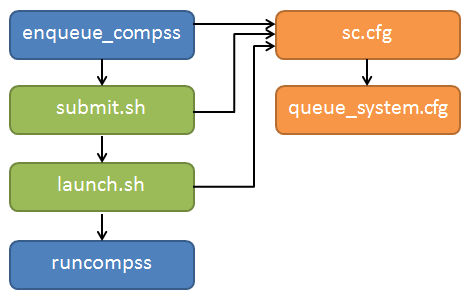
\includegraphics[width=0.6\textwidth]{./Sections/5_Execution_Platforms/Figures/queue_scripts_structure.png}
    \caption{Structure of COMPSs queue scripts. In Blue user scripts, in Green queue scripts and in Orange system dependant scripts}
    \label{fig:queue_scripts_structure}
\end{figure}

To make this structure works, the administrators must define a configuration file for the queue system and a configuration file
for the specific SuperComputer parameters. The COMPSs installation already provides queue configurations for \textit{LSF} and 
\textit{SLURM} and several examples for SuperComputer configurations. 
To create a new configuration we recommend to use one of the configurations provided by COMPSs (such as the configuration for the
\textit{MareNostrum III} SuperComputer) or to contact us at \url{support-compss@bsc.es} .

\subsubsection{MareNostrum III}

For information about how to submit COMPSs applications at MareNostrum III (BSC) please refer to the \textit{COMPSs at BSC} manual 
available at \url{http://compss.bsc.es/releases/compss/latest/docs/COMPSs_MareNostrum_Manual.pdf} .

  
  \section{Common Issues}
\label{sec:Common_Issues}

This section provides answers for the most common issues of the execution of COMPSs applications.
For specific issues not covered in this section, please do not hesitate to contact us at:
\begin{center}
  \textbf{\url{support-compss@bsc.es}}
\end{center}

\subsection{How to debug}
When the application does not behave as expected the first thing users must do is to run it in \textbf{debug} mode executing the \textit{runcompss} command withthe \textit{-d} flag to enable the debug log level.

In this case the application execution will produce the following files:
\begin{itemize}
 \item runtime.log
 \item resources.log
 \item jobs folder
\end{itemize}

First, users should check the last lines of the runtime.log. If the file-transfers or the tasks are failing an error message 
will appear in this file. If the file-transfers are successfully and the jobs are submitted, users should check the \textit{jobs} folder and look 
at the error messages produced inside each job. Users should notice that if there are $\_RESUBMITTED$ files something 
inside the job is failing.

\subsection{Tasks are not executed}
If the tasks remain in \textbf{Blocked} state probably there are no existing resources matching the specific task constraints. 
This error can be potentially caused by two facts: the resources are not correctly loaded into the runtime, or the task constraints do not match with any resource. 

In the first case, users should take a look at the \textit{resouces.log} and check that all the resources
defined in the \textit{project.xml} file are available to the runtime. In the second case users should re-define the task 
constraints taking into account the resources capabilities defined into the \textit{resources.xml} and \textit{project.xml} files.

\subsection{Jobs fail}
If all the application's tasks fail because all the submitted jobs fail, it is probably due to the fact that there is a resource 
miss-configuration. In most of the cases, the resource that the application is trying to access has no passwordless access through
the configured user. This can be checked by:
\begin{itemize}
 \item Open the project.xml. (The default file is stored under \textit{/opt/COMPSs/
 Runtime/configuration/xml/projects/project.xml}
 \item For each resource annotate its name and the value inside the \textit{User} tag. Remember that if there is no \textit{User}
 tag COMPSs will try to connect this resource with the same username than the one that launches the main application.
 \item For each annotated resourceName - user please try \textit{ssh user@resourceName}. If the connection asks for a password then
 there is an error in the configuration of the ssh access in the resource.
\end{itemize}

The problem can be solved running the following commands:
\begin{lstlisting}[language=bash]
compss@bsc:~$ scp ~/.ssh/id_dsa.pub user@resourceName:./mydsa.pub
compss@bsc:~$ ssh user@resourceName "cat mydsa.pub >> ~/.ssh/authorized_keys; rm ./mydsa.pub"
\end{lstlisting}

These commands are a quick solution, for further details please check the \textit{Additional Configuration} section 
inside the \textit{COMPSs Installation Manual} available at our website \url{http://compss.bsc.es}.

\subsection{Compilation error: @Method not found}
When trying to compile Java applications users can get some of the following compilation errors:
\begin{lstlisting}[language=bash]
error: package integratedtoolkit.types.annotations does not exist
import integratedtoolkit.types.annotations.Constraints;
                                          ^
error: package integratedtoolkit.types.annotations does not exist
import integratedtoolkit.types.annotations.Method;
                                          ^
error: package integratedtoolkit.types.annotations does not exist
import integratedtoolkit.types.annotations.Parameter;
                                          ^
error: package integratedtoolkit.types.annotations.Parameter does not exist
import integratedtoolkit.types.annotations.Parameter.Direction;
                                                    ^
error: package integratedtoolkit.types.annotations.Parameter does not exist
import integratedtoolkit.types.annotations.Parameter.Type;
                                                    ^
error: cannot find symbol
@Parameter(type = Type.FILE, direction = Direction.INOUT)
^
  symbol:   class Parameter
  location: interface APPLICATION_Itf
  
error: cannot find symbol
@Constraints(processorCoreCount = 2)
^
  symbol:   class Constraints
  location: interface APPLICATION_Itf
  
error: cannot find symbol
@Method(declaringClass = "application.ApplicationImpl")
^
  symbol:   class Method
  location: interface APPLICATION_Itf
\end{lstlisting}

All these errors are raised because the \textit{compss-engine.jar} is not listed in the CLASSPATH. The default COMPSs installation
automatically inserts this package into the CLASSPATH but it may have been overwritten or deleted. Please check that your 
environment variable CLASSPATH containts the \textit{compss-engine.jar} location by running the following command:
\begin{lstlisting}[language=bash]
$ echo $CLASSPATH | grep compss-engine
\end{lstlisting}
If the result of the previous command is empty it means that you are missing the \textit{compss-engine.jar} package in your classpath. 

The easiest solution is to manually export the CLASSPATH variable into the user session:
\begin{lstlisting}[language=bash]
$ export CLASSPATH=$CLASSPATH:/opt/COMPSs/Runtime/compss-engine.jar
\end{lstlisting}
However, you will need to remember to export this variable every time you log out and back in again. Consequently, we recommend to 
add this export to the \textit{.bashrc} file:
\begin{lstlisting}[language=bash]
$ echo "# COMPSs variables for Java compilation" >> ~/.bashrc
$ echo "export CLASSPATH=$CLASSPATH:/opt/COMPSs/Runtime/compss-engine.jar" >> ~/.bashrc
\end{lstlisting}

\colorComment{Attention: The \textit{compss-engine.jar} is installed inside the COMPSs installation directory. If you have performed
a custom installation, the path of the package may be different.}

\subsection{Jobs failed on method reflection}
When executing an application the main code gets stuck executing a task. Taking a look at the \textit{runtime.log} users can check
that the job associated to the task has failed (and all its resubmissions too). Then, opening the \textit{$jobX\_NEW.out$} or the
\textit{$jobX\_NEW.err$} files users find the following error:

\begin{lstlisting}[language=bash]
[ERROR|integratedtoolkit.Worker|Executor] Can not get method by reflection
integratedtoolkit.nio.worker.executors.Executor$JobExecutionException: Can not get method by reflection
        at integratedtoolkit.nio.worker.executors.JavaExecutor.executeTask(JavaExecutor.java:142)
        at integratedtoolkit.nio.worker.executors.Executor.execute(Executor.java:42)
        at integratedtoolkit.nio.worker.JobLauncher.executeTask(JobLauncher.java:46)
        at integratedtoolkit.nio.worker.JobLauncher.processRequests(JobLauncher.java:34)
        at integratedtoolkit.util.RequestDispatcher.run(RequestDispatcher.java:46)
        at java.lang.Thread.run(Thread.java:745)
Caused by: java.lang.NoSuchMethodException: simple.Simple.increment(java.lang.String)
        at java.lang.Class.getMethod(Class.java:1678)
        at integratedtoolkit.nio.worker.executors.JavaExecutor.executeTask(JavaExecutor.java:140)
        ... 5 more
\end{lstlisting}

This error is due to the fact that COMPSs cannot find one of the tasks declared in the Java Interface. Commonly this is triggered by
one of the following errors:

\begin{itemize}
 \item The \textit{declaringClass} of the tasks in the Java Interface has not been correctly defined.
 \item The parameters of the tasks in the Java Interface do not match the task call.
 \item The tasks have not been defined as \textit{public}.
\end{itemize}

\subsection{Jobs failed on reflect target invocation null pointer}
When executing an application the main code gets stuck executing a task. Taking a look at the \textit{runtime.log} users can check
that the job associated to the task has failed (and all its resubmissions too). Then, opening the \textit{$jobX\_NEW.out$} or the
\textit{$jobX\_NEW.err$} files users find the following error:

\begin{lstlisting}[language=bash]
[ERROR|integratedtoolkit.Worker|Executor]
java.lang.reflect.InvocationTargetException
        at sun.reflect.NativeMethodAccessorImpl.invoke0(Native Method)
        at sun.reflect.NativeMethodAccessorImpl.invoke(NativeMethodAccessorImpl.java:57)
        at sun.reflect.DelegatingMethodAccessorImpl.invoke(DelegatingMethodAccessorImpl.java:43)
        at java.lang.reflect.Method.invoke(Method.java:606)
        at integratedtoolkit.nio.worker.executors.JavaExecutor.executeTask(JavaExecutor.java:154)
        at integratedtoolkit.nio.worker.executors.Executor.execute(Executor.java:42)
        at integratedtoolkit.nio.worker.JobLauncher.executeTask(JobLauncher.java:46)
        at integratedtoolkit.nio.worker.JobLauncher.processRequests(JobLauncher.java:34)
        at integratedtoolkit.util.RequestDispatcher.run(RequestDispatcher.java:46)
        at java.lang.Thread.run(Thread.java:745)
Caused by: java.lang.NullPointerException
        at simple.Ll.printY(Ll.java:25)
        at simple.Simple.task(Simple.java:72)
        ... 10 more
\end{lstlisting}

This cause of this error is that the Java object accessed by the task has not been correctly transferred and one or more of its fields
is null. The transfer failure is normally caused because the transferred object is not serializable. 

Users should check that all the object parameters in the task are either implementing the serializable interface or following 
the \textit{java beans} model (by implementing an empty constructor and getters and setters for each attribute).


  %%%%%%%%%%%%% END PAGE %%%%%%%%%%%%%%
  \newpage

  \vspace*{\fill} 
  \begin{center}
    \large { Please find more details on the COMPSs framework at }
    \huge{\url{http://compss.bsc.es}}
  \end{center}    
  \vspace*{\fill} 
           
\end{document}
